% Figure snippets, included inline in main.tex.

\begin{figure}[t]
  \centering
  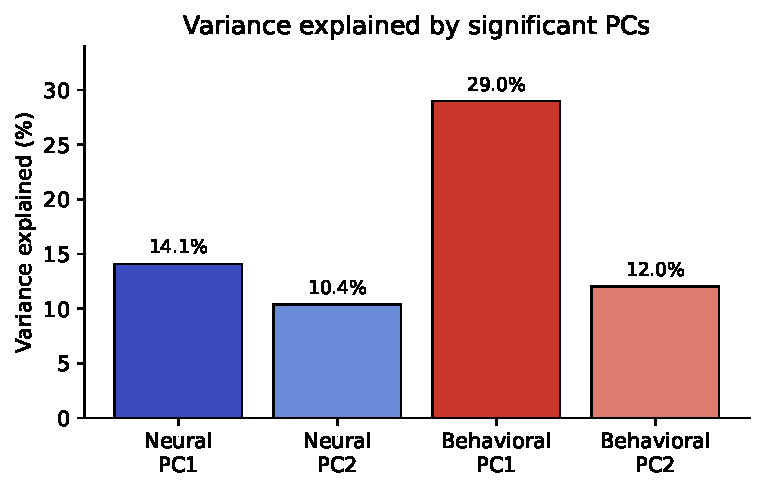
\includegraphics[width=0.80\linewidth]{figures/fig1_variance.pdf}
  \caption{\textbf{Ketamine produces multidimensional neural and behavioral effects.}
  Variance explained by the significant principal components obtained from
  (left) PCA on $\Delta$GBC across 718 functionally-defined parcels and
  (right) PCA on 31 behavioral measures. The first two neural PCs
  capture 14.1\% and 10.4\% of neural variance, respectively. The first two
  behavioral PCs capture 29.0\% and 12.0\%. Five neural PCs were significant
  by permutation test ($p<0.05$, 5000 permutations), together capturing
  42.1\% of neural variance; two behavioral PCs were significant, together
  capturing 41.1\% of behavioral variance.}
  \label{fig:variance}
\end{figure}

\begin{figure}[t]
  \centering
  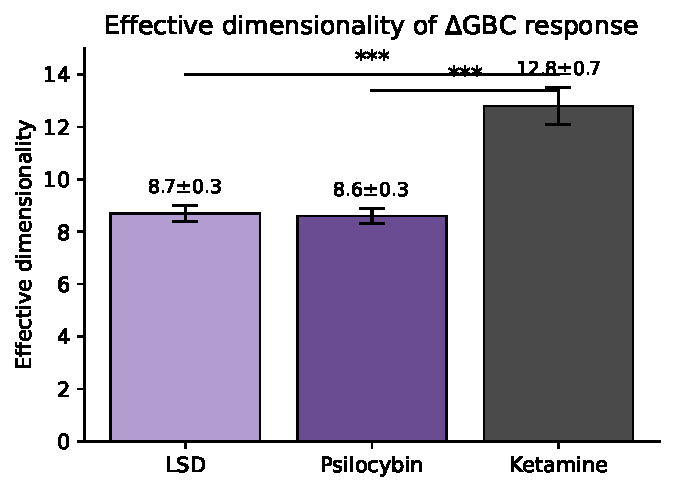
\includegraphics[width=0.72\linewidth]{figures/fig2_dimensionality.pdf}
  \caption{\textbf{Ketamine's $\Delta$GBC response is higher-dimensional than
  LSD's or psilocybin's.} Effective neural dimensionality of the $\Delta$GBC
  response across three psychoactive pharmacological conditions. Ketamine
  (12.8$\pm$0.7) is significantly higher-dimensional than both LSD
  (8.7$\pm$0.3) and psilocybin (8.6$\pm$0.3) (one-way ANOVA
  $F(2,60)=564$, $p<0.001$; post-hoc $p<0.001$ for both contrasts,
  Bonferroni corrected). LSD and psilocybin do not differ significantly
  from each other ($p=0.6$).}
  \label{fig:dimensionality}
\end{figure}

\begin{figure}[t]
  \centering
  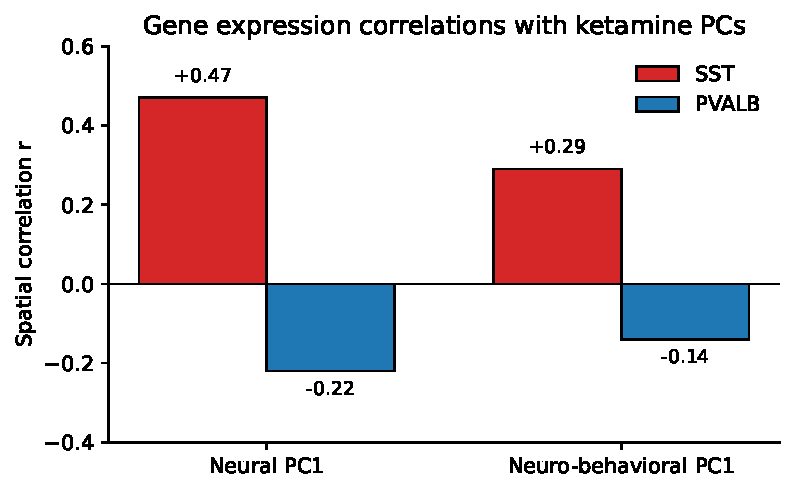
\includegraphics[width=0.80\linewidth]{figures/fig3_gene_corr.pdf}
  \caption{\textbf{The leading ketamine gradient tracks interneuron cell-type
  gene expression.} Spatial correlation between SST (red) and PVALB (blue)
  cortical gene expression maps and (left) the leading neural PC1 $\Delta$GBC
  map, and (right) the leading neuro-behavioral PC1 map. For neural PC1,
  SST $r=0.47$ ($p<0.001$) and PVALB $r=-0.22$ ($p=0.025$). For
  neuro-behavioral PC1, SST $r=0.29$ ($p=0.009$) and PVALB $r=-0.14$
  ($p=0.089$). All $p$ values are from 100{,}000 spatial-null permutations.}
  \label{fig:gene}
\end{figure}

\begin{figure}[t]
  \centering
  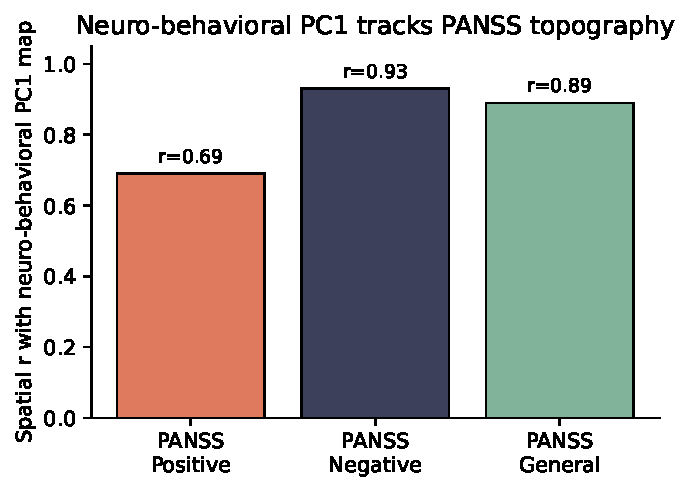
\includegraphics[width=0.72\linewidth]{figures/fig4_panss_map_corr.pdf}
  \caption{\textbf{Neuro-behavioral PC1 recapitulates clinical symptom
  topography.} Spatial correlation across 718 parcels between the
  neuro-behavioral PC1 map and the three PANSS subscale maps:
  Positive ($r=0.69$), Negative ($r=0.93$), and General ($r=0.89$);
  all $p<0.001$, $n=718$ parcels.}
  \label{fig:panss}
\end{figure}
